\section{Observations}\label{sec:observations}

% make interesting observations about the data.
% Document how you came to these observations
% and how the application design was beneficial (or not) to your discoveries.
% Emphasize on interaction aspects, and also
% explain why you think your approach is good from a perceptual point of view
% and how it takes design principles into account (slides!).
% Provide some support by citing relevant literature.



With the application fully implemented, we will use it to perform the tasks that were defined in Section \ref{subsec:chosentasks}, and will evaluate how suitable the application is for completing these tasks. We start with the first specific question of the first. For convenience we list the specific questions of the first task once more:

Do restaurants receive a better rating when they
\begin{enumerate}
\setlength{\itemsep}{0cm}%
\setlength{\parskip}{0cm}%
\item are part of a franchise?
\item provide internet?
\item serve a certain cuisine?
\item are located in a certain area?
\end{enumerate}

%%task1 Q1
%%seems to be that better rating when not part of franchise
%%HOWEVER, is quantitative, not qualitative
For question 1 use the PCP and set its restaurant attribute to franchise (the consumer attribute can be arbitrary). We then filter this attribute on either true or false, and filter the rating on value 2. If we now switch the franchise filter from true to false, we see on the map that there are much more restaurants that are not part of a franchise that have received a rating of 2, than restaurant that are part of a franchise (sse Figure \ref{fig:task1q1}. This might indicate that restaurants that are not part of a franchise receive better ratings in general. However, this observation is only a quantitative one. It might for instance be that much less restaurants that are part of a franchise got reviewed at all, and therefore have less ratings of value 2. Then again, the fact that these restaurant get rated less often may also say something about their popularity.

\begin{figure}[h]
    \centering
    \captionsetup{justification=centering,margin=0.5cm}
    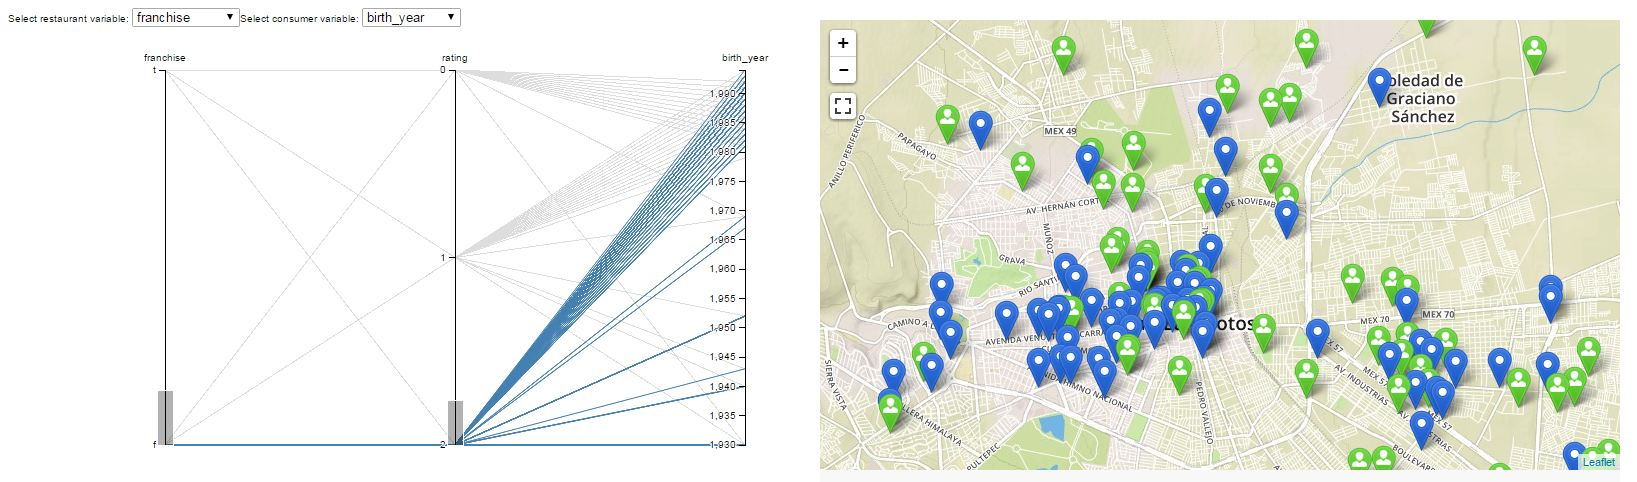
\includegraphics[width=.8\textwidth]{img/task1q1a.jpg}
    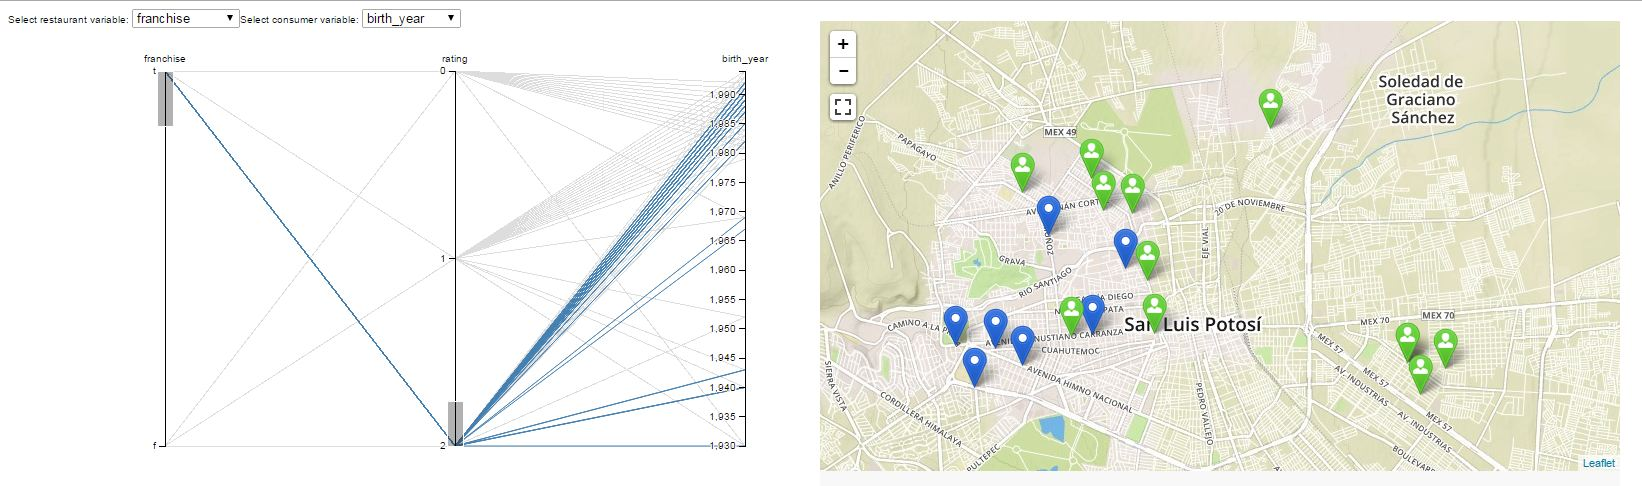
\includegraphics[width=.8\textwidth]{img/task1q1b.jpg}
    \caption{Comparison of restaurants that are \emph{not} part of a franchise and received a rating of value 2 (upper image) with restaurants that are part of a franchise and received a rating of value 2 (lower image).}
    \label{fig:task1q1}
\end{figure}

%%task1 Q2
For question 2 we can take a similar approach as with question 1: we set the restaurant attribute to 'Other Services', filter on 'Internet', and then compare the ratings these restaurants received by consecutively filtering the rating axis on the values 0, 1 and 2. This reveals that around the city of Cuernavaca, restaurants that provide internet, are more often rated with a value of 2 (see Figure \ref{fig:task1q2}).

\begin{figure}[h]
    \centering
    \captionsetup{justification=centering,margin=0.5cm}
    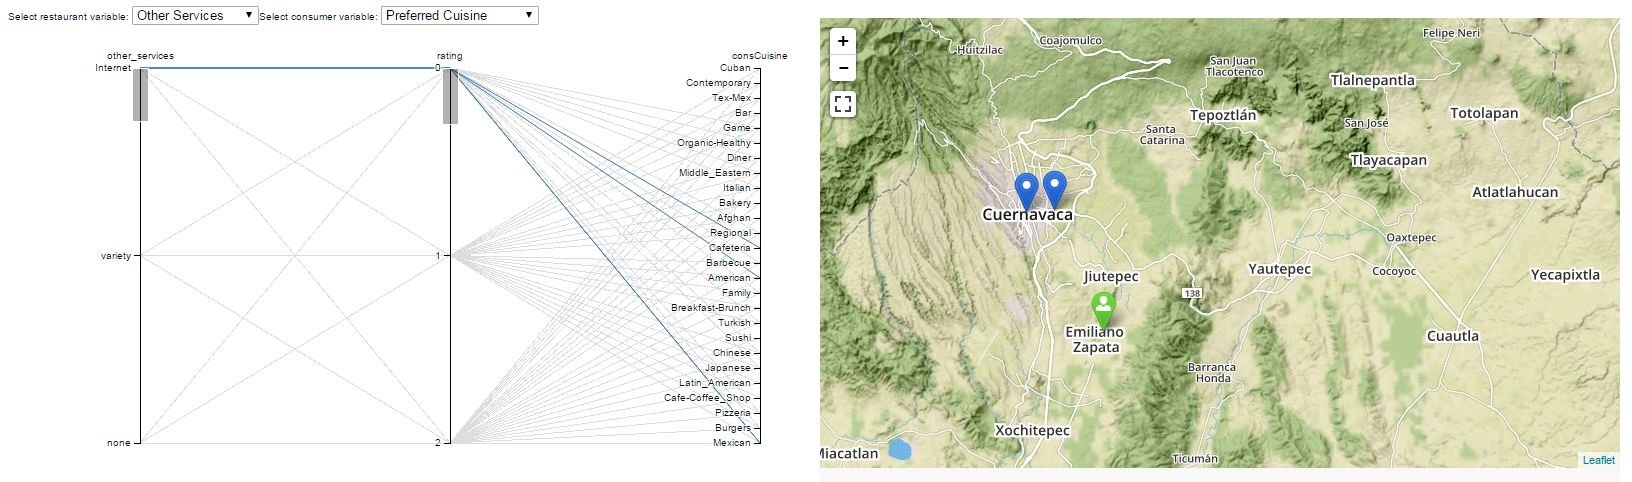
\includegraphics[width=.8\textwidth]{img/task1q2a.jpg}
    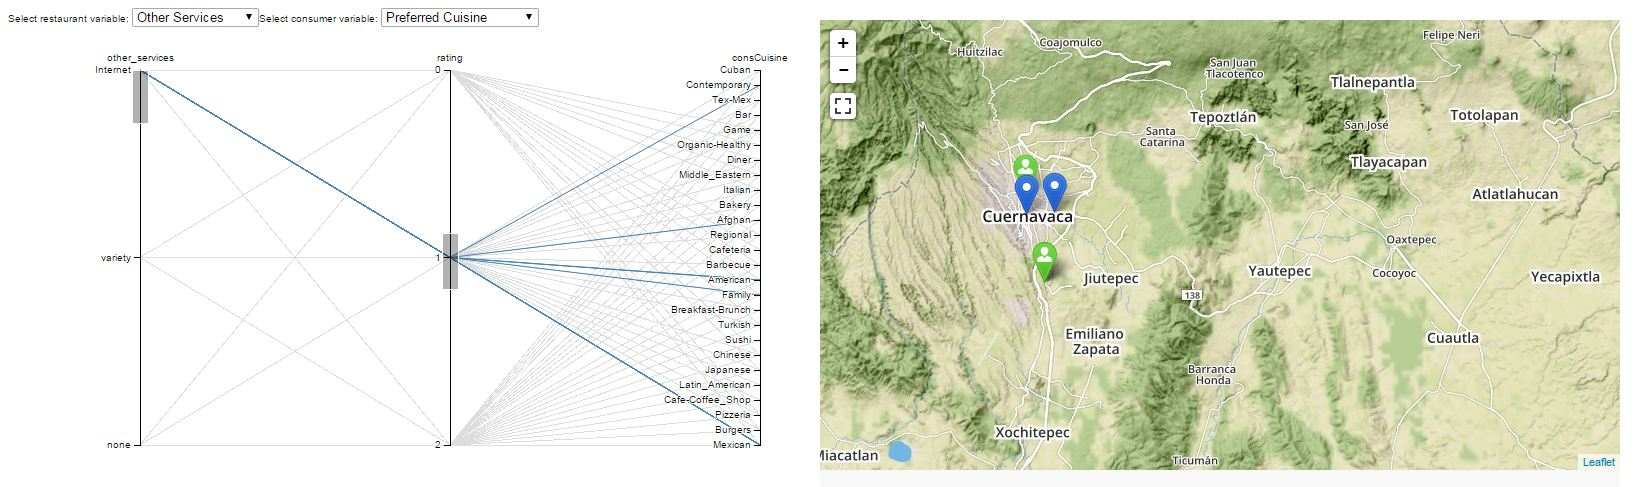
\includegraphics[width=.8\textwidth]{img/task1q2b.jpg}
    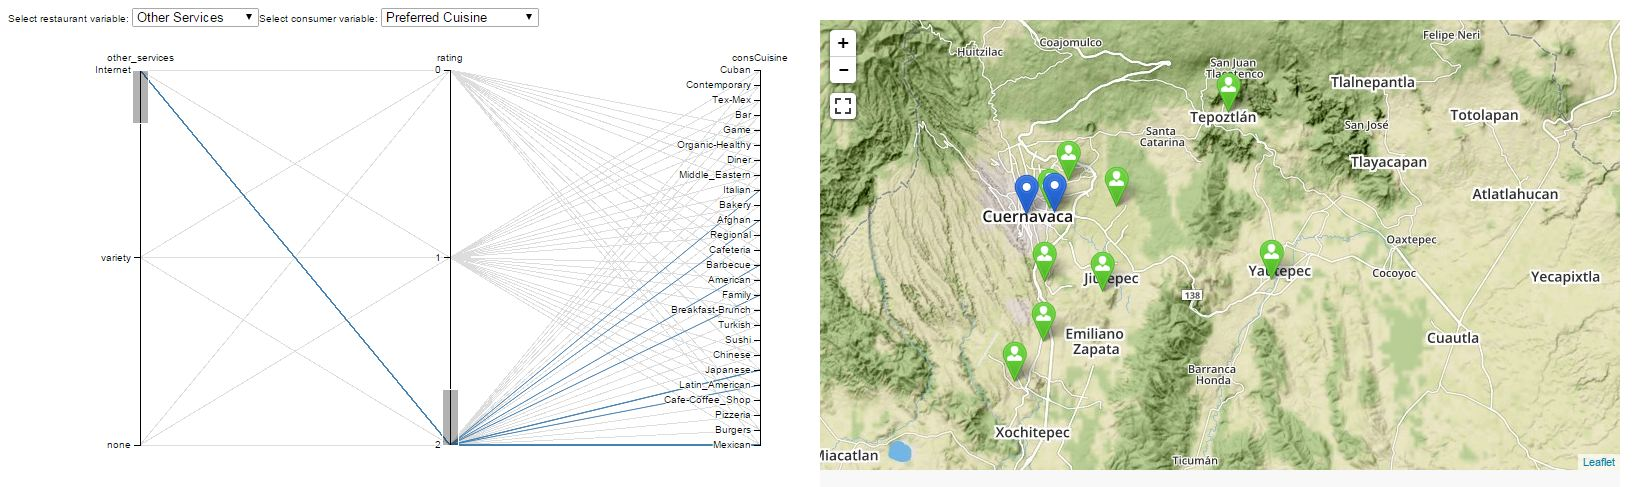
\includegraphics[width=.8\textwidth]{img/task1q2c.jpg}
    \caption{Comparison of the rating values received by restaurants that provide internet.}
    \label{fig:task1q2}
\end{figure}

%%task1 Q3
When applying the approach of question 2 to question 3, we are not able to draw any clear conclusions. The only observations that we can make is that (the only) restaurant with a Regional cuisine never got a rating of 2 (by the two consumers that rated it), while restaurants of the cuisines Coffee (1 restaurant, rated by twelve consumers), Armenian (1 restaurant, rated by four consumers) and Contemporary (again 1 restaurant, rated by four consumers) never get a rating value of 0. The only Bar/Pub (rated by five consumers) even received only rating values of 2. In conclusion, we can say something about clear outliers regarding this question, although it needs some additional exploration of the map.

%%task1 Q4
...

%%task2a Q1
%%just see that less people in general visit restaurants that are part of franchise
...

%%task2a Q2
%%Seems like it: Jewish people only went to few types of restaurants. HOWEVER, could be that there are only very few jewish consumers. Further investigation (i.e., exploring the map) indeed shows there is only one jewish consumer that visited eight differnet restaurants. Same holds for Mormon. Christian bit more interesting: about 7 consumers that do not visit more than half of the cuisines (including chinese, Armenian, Japanese, Burgers, etc.)
...

%%task2b Q1
%%no real correlation smoker - not permitted
...

%%task2b Q2
%%no record of consumers that drink a lot. only social. But again go to a lot of non-alcoholic restaurants and rate them good
...

%%task2b Q3
%%especially vry few high budget - low price occurrences. But they still rate them weel though (we do need to take quite some exploring to find this out: set pcp, browse map en manually count.
...

%%task 2b Q4
%%yes some do. According to data even someone that rated about ten restaurants far away that transports himself by foot -> can't be right
%%also: quite some people with a car go to restaurant without parking lot. Does not need to say anything though: may not always go by car
...


\subsection{Improvements}\label{sec:improvements}
- display the total number of selected lines in the PCP
\\- ...






